\chapter{Camins més curts}

\index{camí més curt}

Trobar el camí més curt entre dos nodes d'un graf és un problema
important que té moltes aplicacions pràctiques. Per exemple, donada
una xarxa de carreteres, calcula la longitud més curta possible d'una
ruta entre dues ciutats, tenint en compte les longituds de les
carreteres.

En un graf sense pesos, la longitud d'un camí és igual al nombre
d'arestes, i podem fer servir la cerca en amplada per trobar el camí
més curt. Tanmateix, en aquest capítol ens centrem en els grafs amb
pesos on necessitem algorismes més sofisticats per trobar els camins
mínims.

\section{Algorisme de Bellman–Ford}

\index{Algorisme de Bellman–Ford}

L'\key{algorisme de Bellman–Ford}\footnote{L'algorisme rep el nom de
R.E. Bellman i L.R. Ford que el van publicar de manera independentment
els anys 1958 i el 1956 \cite{bel58,for56a}.} troba els camins més
curts des d'un node inicial a tots els nodes del graf. L'algorisme pot
processar tot tipus de grafs, sempre que el graf no contingui un cicle
de longitud negativa. L'algorisme és capaç de detectar si el graf té
cicles de longitud negativa.

L'algorisme manté un vector amb les millors distàncies conegudes des
del node inicial fins a tots els nodes del graf. Inicialment, la
distància al node inicial és 0 i la distància a tots els altres nodes
és infinita. L'algorisme redueix les distàncies trobant arestes que
escurcen els camins fins que no és possible reduir cap distància.

\subsubsection{Exemple}

Mostrem com funciona l'algorisme de Bellman-Ford en el graf següent:
\begin{center}
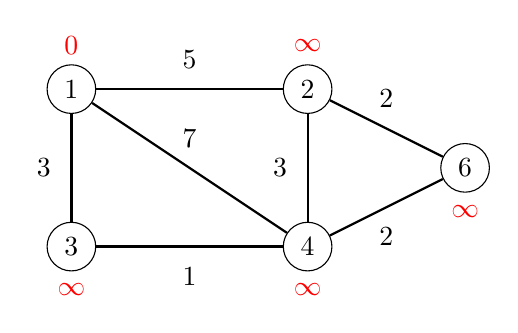
\begin{tikzpicture}
\node[draw, circle] (1) at (1,3) {1};
\node[draw, circle] (2) at (4,3) {2};
\node[draw, circle] (3) at (1,1) {3};
\node[draw, circle] (4) at (4,1) {4};
\node[draw, circle] (5) at (6,2) {6};
\node[color=red] at (1,3+0.55) {$0$};
\node[color=red] at (4,3+0.55) {$\infty$};
\node[color=red] at (1,1-0.55) {$\infty$};
\node[color=red] at (4,1-0.55) {$\infty$};
\node[color=red] at (6,2-0.55) {$\infty$};
\path[draw,thick,-] (1) -- node[font=\small,label=above:5] {} (2);
\path[draw,thick,-] (1) -- node[font=\small,label=left:3] {} (3);
\path[draw,thick,-] (3) -- node[font=\small,label=below:1] {} (4);
\path[draw,thick,-] (2) -- node[font=\small,label=left:3] {} (4);
\path[draw,thick,-] (2) -- node[font=\small,label=above:2] {} (5);
\path[draw,thick,-] (4) -- node[font=\small,label=below:2] {} (5);
\path[draw,thick,-] (1) -- node[font=\small,label=above:7] {} (4);
\end{tikzpicture}
\end{center}
A cada node del graf li assignem una distància. Inicialment, la
distància al node inicial és 0 i la distància a tots els altres nodes
és infinita.

L'algorisme cerca arestes que redueixin distàncies. En primer lloc,
totes les arestes del node 1 redueixen les distàncies:
\begin{center}
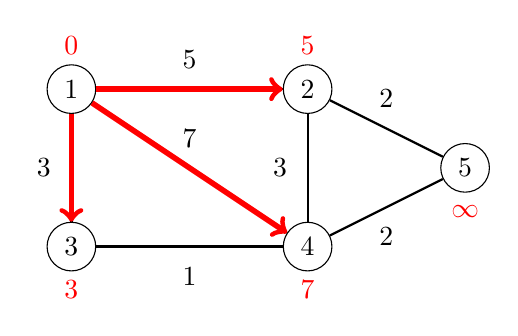
\begin{tikzpicture}
\node[draw, circle] (1) at (1,3) {1};
\node[draw, circle] (2) at (4,3) {2};
\node[draw, circle] (3) at (1,1) {3};
\node[draw, circle] (4) at (4,1) {4};
\node[draw, circle] (5) at (6,2) {5};
\node[color=red] at (1,3+0.55) {$0$};
\node[color=red] at (4,3+0.55) {$5$};
\node[color=red] at (1,1-0.55) {$3$};
\node[color=red] at (4,1-0.55) {$7$};
\node[color=red] at (6,2-0.55) {$\infty$};
\path[draw,thick,-] (1) -- node[font=\small,label=above:5] {} (2);
\path[draw,thick,-] (1) -- node[font=\small,label=left:3] {} (3);
\path[draw,thick,-] (3) -- node[font=\small,label=below:1] {} (4);
\path[draw,thick,-] (2) -- node[font=\small,label=left:3] {} (4);
\path[draw,thick,-] (2) -- node[font=\small,label=above:2] {} (5);
\path[draw,thick,-] (4) -- node[font=\small,label=below:2] {} (5);
\path[draw,thick,-] (1) -- node[font=\small,label=above:7] {} (4);

\path[draw=red,thick,->,line width=2pt] (1) -- (2);
\path[draw=red,thick,->,line width=2pt] (1) -- (3);
\path[draw=red,thick,->,line width=2pt] (1) -- (4);
\end{tikzpicture}
\end{center}
Després d'això, les arestes $2 \rightarrow 5$ i $3 \rightarrow 4$
redueixen les distàncies:
\begin{center}
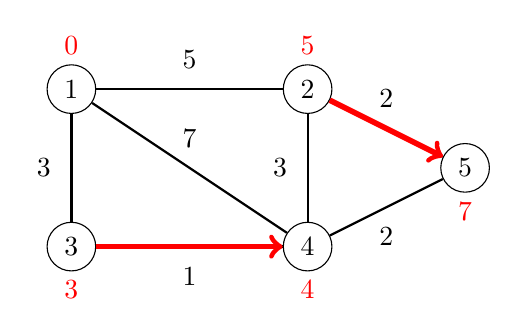
\begin{tikzpicture}
\node[draw, circle] (1) at (1,3) {1};
\node[draw, circle] (2) at (4,3) {2};
\node[draw, circle] (3) at (1,1) {3};
\node[draw, circle] (4) at (4,1) {4};
\node[draw, circle] (5) at (6,2) {5};
\node[color=red] at (1,3+0.55) {$0$};
\node[color=red] at (4,3+0.55) {$5$};
\node[color=red] at (1,1-0.55) {$3$};
\node[color=red] at (4,1-0.55) {$4$};
\node[color=red] at (6,2-0.55) {$7$};
\path[draw,thick,-] (1) -- node[font=\small,label=above:5] {} (2);
\path[draw,thick,-] (1) -- node[font=\small,label=left:3] {} (3);
\path[draw,thick,-] (3) -- node[font=\small,label=below:1] {} (4);
\path[draw,thick,-] (2) -- node[font=\small,label=left:3] {} (4);
\path[draw,thick,-] (2) -- node[font=\small,label=above:2] {} (5);
\path[draw,thick,-] (4) -- node[font=\small,label=below:2] {} (5);
\path[draw,thick,-] (1) -- node[font=\small,label=above:7] {} (4);

\path[draw=red,thick,->,line width=2pt] (2) -- (5);
\path[draw=red,thick,->,line width=2pt] (3) -- (4);
\end{tikzpicture}
\end{center}
Finalment, hi ha un canvi més:
\begin{center}
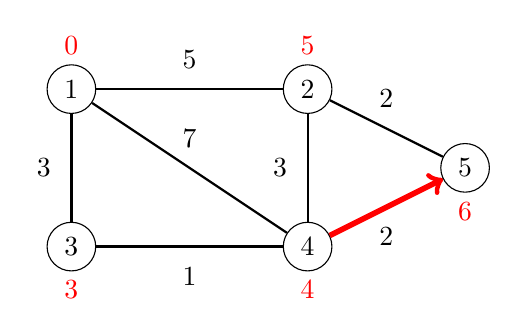
\begin{tikzpicture}
\node[draw, circle] (1) at (1,3) {1};
\node[draw, circle] (2) at (4,3) {2};
\node[draw, circle] (3) at (1,1) {3};
\node[draw, circle] (4) at (4,1) {4};
\node[draw, circle] (5) at (6,2) {5};
\node[color=red] at (1,3+0.55) {$0$};
\node[color=red] at (4,3+0.55) {$5$};
\node[color=red] at (1,1-0.55) {$3$};
\node[color=red] at (4,1-0.55) {$4$};
\node[color=red] at (6,2-0.55) {$6$};
\path[draw,thick,-] (1) -- node[font=\small,label=above:5] {} (2);
\path[draw,thick,-] (1) -- node[font=\small,label=left:3] {} (3);
\path[draw,thick,-] (3) -- node[font=\small,label=below:1] {} (4);
\path[draw,thick,-] (2) -- node[font=\small,label=left:3] {} (4);
\path[draw,thick,-] (2) -- node[font=\small,label=above:2] {} (5);
\path[draw,thick,-] (4) -- node[font=\small,label=below:2] {} (5);
\path[draw,thick,-] (1) -- node[font=\small,label=above:7] {} (4);

\path[draw=red,thick,->,line width=2pt] (4) -- (5);
\end{tikzpicture}
\end{center}


Després d'això, cap aresta pot reduir cap distància. Això vol dir que
les distàncies són definitives i hem calculat correctament les
distàncies més curtes des del node inicial fins a tots els nodes del
graf.

Per exemple, la distància més curta del node 1 al node 5 és 3 i es
correspon amb al camí següent:


\begin{center}
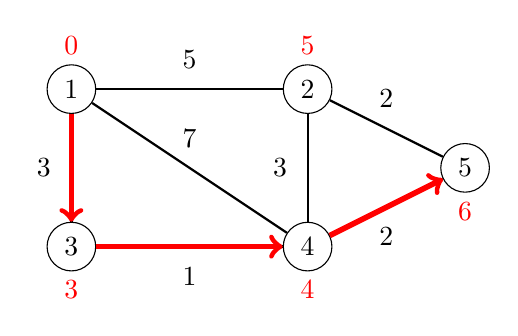
\begin{tikzpicture}
\node[draw, circle] (1) at (1,3) {1};
\node[draw, circle] (2) at (4,3) {2};
\node[draw, circle] (3) at (1,1) {3};
\node[draw, circle] (4) at (4,1) {4};
\node[draw, circle] (5) at (6,2) {5};
\node[color=red] at (1,3+0.55) {$0$};
\node[color=red] at (4,3+0.55) {$5$};
\node[color=red] at (1,1-0.55) {$3$};
\node[color=red] at (4,1-0.55) {$4$};
\node[color=red] at (6,2-0.55) {$6$};
\path[draw,thick,-] (1) -- node[font=\small,label=above:5] {} (2);
\path[draw,thick,-] (1) -- node[font=\small,label=left:3] {} (3);
\path[draw,thick,-] (3) -- node[font=\small,label=below:1] {} (4);
\path[draw,thick,-] (2) -- node[font=\small,label=left:3] {} (4);
\path[draw,thick,-] (2) -- node[font=\small,label=above:2] {} (5);
\path[draw,thick,-] (4) -- node[font=\small,label=below:2] {} (5);
\path[draw,thick,-] (1) -- node[font=\small,label=above:7] {} (4);

\path[draw=red,thick,->,line width=2pt] (1) -- (3);
\path[draw=red,thick,->,line width=2pt] (3) -- (4);
\path[draw=red,thick,->,line width=2pt] (4) -- (5);
\end{tikzpicture}
\end{center}


\subsubsection{Implementació}

La següent implementació de l'algorisme de Bellman-Ford determina les
distàncies més curtes des d'un node $x$ a tots els nodes del graf. El
codi suposa que el graf s'emmagatzema com una llista de arestes
\texttt{edges} que consta de tuples de la forma $(a,b,w)$, el que
significa que hi ha una aresta des del node $a$ fins al node $b$ amb
pes $w$.

L'algorisme consta de $n-1$ rondes, i a cada ronda l'algoritme passa
per totes les arestes del graf i intenta reduir les
distàncies. L'algorisme construeix una vector \texttt{distance} que
conté les millors distàncies conegudes de $x$ a tots els nodes del
graf. La constant \texttt{INF} denota una distància infinita.


\begin{lstlisting}
for (int i = 1; i <= n; i++) distance[i] = INF;
distance[x] = 0;
for (int i = 1; i <= n-1; i++) {
    for (auto e : edges) {
        int a, b, w;
        tie(a, b, w) = e;
        distance[b] = min(distance[b], distance[a]+w);
    }
}
\end{lstlisting}


La complexitat temporal de l'algorisme és $O(nm)$, perquè l'algoritme
consta de $n-1$ rondes i itera per totes les $m$ arestes durant una
ronda. Si no hi ha cicles negatius al graf, totes les distàncies són
finals després de $n-1$ rondes, perquè els camins mínims no poden
repetir nodes, i per tant contenen com a molt $n-1$ arestes.

A la pràctica, sovint no és necessari fer $n-1$ rondes per a trobar
les distàncies definitives. Podem fer l'algorsime més eficent si
l'aturem quan no reduim cap distància durant una ronda.

\subsubsection{Cicles negatius}

\index{cicle negatiu}

L'algorisme de Bellman-Ford també es pot fer servir per comprovar si
el graf conté un cicle de longitud negativa. Per exemple, el graf


\begin{center}
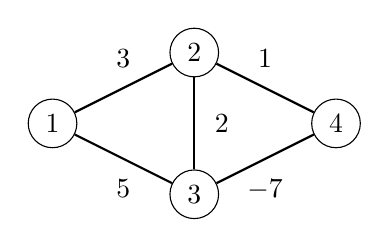
\begin{tikzpicture}[scale=0.9]
\node[draw, circle] (1) at (0,0) {$1$};
\node[draw, circle] (2) at (2,1) {$2$};
\node[draw, circle] (3) at (2,-1) {$3$};
\node[draw, circle] (4) at (4,0) {$4$};

\path[draw,thick,-] (1) -- node[font=\small,label=above:$3$] {} (2);
\path[draw,thick,-] (2) -- node[font=\small,label=above:$1$] {} (4);
\path[draw,thick,-] (1) -- node[font=\small,label=below:$5$] {} (3);
\path[draw,thick,-] (3) -- node[font=\small,label=below:$-7$] {} (4);
\path[draw,thick,-] (2) -- node[font=\small,label=right:$2$] {} (3);
\end{tikzpicture}
\end{center}
\noindent conté un cicle negatiu $2 \rightarrow 3 \rightarrow 4
\rightarrow 2$ de longitud $-4$.

Si el graf conté un cicle negatiu, podem escurçar infinites vegades
qualsevol camí que contingui el cicle repetint el cicle una i altra
vegada. Per tant, el concepte de camí més curt no té sentit en aquesta
situació.

Podem detectar ciclces negatius executant l'algorisme de Bellman-Ford
exactament $n$ rondes. Si l'última ronda redueix alguna distància, el
graf conté un cicle negatiu. Observeu que aquest algorisme es pot fer
servir per cercar un cicle negatiu a tot el graf independentment del
node inicial.

\subsubsection{Algorisme SPFA}

\index{Algorisme SPFA}

L'algorisme \key{SPFA} (''Shortest Path Faster Algorithm'')
\cite{fan94} és una variant de l'algorisme de Bellman–Ford, que sovint
és més eficient que l'algorisme original. L'algoritme SPFA no passa
per totes les arestes a cada ronda, sinó que tria les arestes que
s'han d'examinar d'una manera més intel·ligent.

L'algorisme manté una cua de nodes que es poden fer servir per reduir
les distàncies. En primer lloc, l'algoritme afegeix el node inicial
$x$ a la cua. A continuació, l'algorisme considera el primer node $a$
de la cua, i comprova si les arestes de la forma $a \rightarrow b$
redueixen la distància, i si és el cas, afegeix el node $b$ a la cua.

L'eficiència de l'algorisme SPFA depèn de l'estructura del graf:
l'algorisme és sovint eficient, però la seva complexitat temporal en
el pitjor dels casos segueix sent $O(nm)$ i és possible crear entrades
que fan que l'algorisme sigui tan lent com l'algorisme original de
Bellman-Ford.

\section{Algorisme de Dijkstra}

\index{Algorisme de Dijkstra}

\key{Algorisme de Dijkstra}\footnote{E. W. Dijkstra va publicar
l'algorisme el 1959 \cite{dij59}; tanmateix, el seu article original
no esmenta com implementar l'algorisme de manera eficient.} troba els
camins més curts des del node inicial fins a tots els nodes del graf,
a l'igual que l'algorisme de Bellman-Ford. L'avantatge de l'algorisme de
Dijsktra és que és més eficient i es pot fer servir per processar grafs
grans. Tanmateix, l'algorisme requereix que no hi hagi arestes de pes
negatius al graf.

Igual que l'algorisme de Bellman-Ford, l'algoritme de Dijkstra manté
les distàncies als nodes i les redueix durant la cerca. L'algorisme de
Dijkstra és eficient, perquè només processa cada aresta del graf una
vegada, fent servir el fet que no hi ha arestes negatives.

\subsubsection{Exemple}

Considerem com funciona l'algorisme de Dijkstra al graf següent quan
el node inicial és el node 1:
\begin{center}
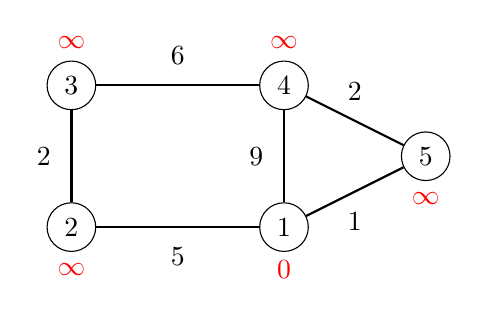
\begin{tikzpicture}[scale=0.9]
\node[draw, circle] (1) at (1,3) {3};
\node[draw, circle] (2) at (4,3) {4};
\node[draw, circle] (3) at (1,1) {2};
\node[draw, circle] (4) at (4,1) {1};
\node[draw, circle] (5) at (6,2) {5};

\node[color=red] at (1,3+0.6) {$\infty$};
\node[color=red] at (4,3+0.6) {$\infty$};
\node[color=red] at (1,1-0.6) {$\infty$};
\node[color=red] at (4,1-0.6) {$0$};
\node[color=red] at (6,2-0.6) {$\infty$};

\path[draw,thick,-] (1) -- node[font=\small,label=above:6] {} (2);
\path[draw,thick,-] (1) -- node[font=\small,label=left:2] {} (3);
\path[draw,thick,-] (3) -- node[font=\small,label=below:5] {} (4);
\path[draw,thick,-] (2) -- node[font=\small,label=left:9] {} (4);
\path[draw,thick,-] (2) -- node[font=\small,label=above:2] {} (5);
\path[draw,thick,-] (4) -- node[font=\small,label=below:1] {} (5);
\end{tikzpicture}
\end{center}
A l'igual que en l'algorisme de Bellman-Ford, inicialment la distància
al node inicial és 0 i la distància a tots els altres nodes és
infinita.

A cada pas, l'algoritme de Dijkstra selecciona aquell node que encara no
s'ha processat i que està a distància mínima. El primer d'aquests
nodes és el node 1 a distància 0.

Quan es selecciona un node, l'algoritme passa per totes les arestes
que surten del node i redueix les distàncies:
\begin{center}
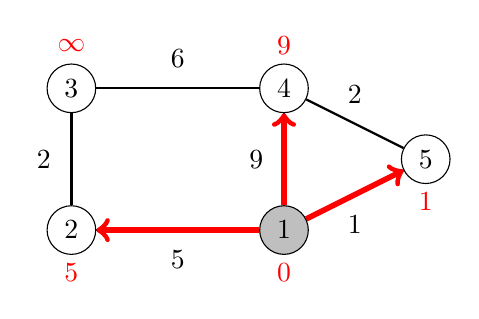
\begin{tikzpicture}[scale=0.9]
\node[draw, circle] (1) at (1,3) {3};
\node[draw, circle] (2) at (4,3) {4};
\node[draw, circle] (3) at (1,1) {2};
\node[draw, circle, fill=lightgray] (4) at (4,1) {1};
\node[draw, circle] (5) at (6,2) {5};

\node[color=red] at (1,3+0.6) {$\infty$};
\node[color=red] at (4,3+0.6) {$9$};
\node[color=red] at (1,1-0.6) {$5$};
\node[color=red] at (4,1-0.6) {$0$};
\node[color=red] at (6,2-0.6) {$1$};

\path[draw,thick,-] (1) -- node[font=\small,label=above:6] {} (2);
\path[draw,thick,-] (1) -- node[font=\small,label=left:2] {} (3);
\path[draw,thick,-] (3) -- node[font=\small,label=below:5] {} (4);
\path[draw,thick,-] (2) -- node[font=\small,label=left:9] {} (4);
\path[draw,thick,-] (2) -- node[font=\small,label=above:2] {} (5);
\path[draw,thick,-] (4) -- node[font=\small,label=below:1] {} (5);

\path[draw=red,thick,->,line width=2pt] (4) -- (2);
\path[draw=red,thick,->,line width=2pt] (4) -- (3);
\path[draw=red,thick,->,line width=2pt] (4) -- (5);
\end{tikzpicture}
\end{center}
En aquest cas, les arestes del node 1 redueixen les distàncies als
nodes 2, 4 i 5, que passen a ser ara 5, 9 i 1.

El següent node a processar és el node 5 a distància 1. Això redueix
la distància al node 4 de 9 a 3:
\begin{center}
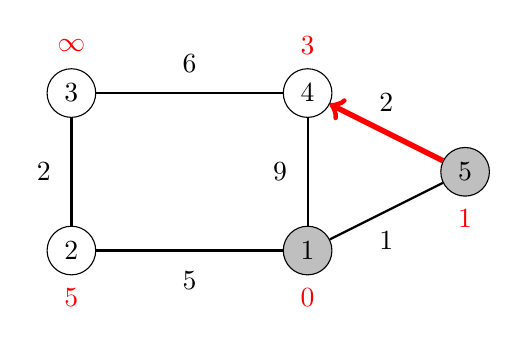
\begin{tikzpicture}
\node[draw, circle] (1) at (1,3) {3};
\node[draw, circle] (2) at (4,3) {4};
\node[draw, circle] (3) at (1,1) {2};
\node[draw, circle, fill=lightgray] (4) at (4,1) {1};
\node[draw, circle, fill=lightgray] (5) at (6,2) {5};

\node[color=red] at (1,3+0.6) {$\infty$};
\node[color=red] at (4,3+0.6) {$3$};
\node[color=red] at (1,1-0.6) {$5$};
\node[color=red] at (4,1-0.6) {$0$};
\node[color=red] at (6,2-0.6) {$1$};

\path[draw,thick,-] (1) -- node[font=\small,label=above:6] {} (2);
\path[draw,thick,-] (1) -- node[font=\small,label=left:2] {} (3);
\path[draw,thick,-] (3) -- node[font=\small,label=below:5] {} (4);
\path[draw,thick,-] (2) -- node[font=\small,label=left:9] {} (4);
\path[draw,thick,-] (2) -- node[font=\small,label=above:2] {} (5);
\path[draw,thick,-] (4) -- node[font=\small,label=below:1] {} (5);

\path[draw=red,thick,->,line width=2pt] (5) -- (2);
\end{tikzpicture}
\end{center}

Després d'això, el següent node és el node 4, i fa que la distància
al node 3 sigui 9:
\begin{center}
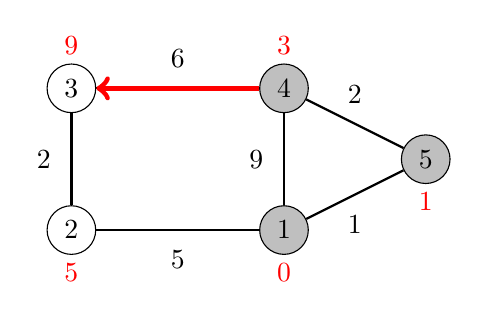
\begin{tikzpicture}[scale=0.9]
\node[draw, circle] (1) at (1,3) {3};
\node[draw, circle, fill=lightgray] (2) at (4,3) {4};
\node[draw, circle] (3) at (1,1) {2};
\node[draw, circle, fill=lightgray] (4) at (4,1) {1};
\node[draw, circle, fill=lightgray] (5) at (6,2) {5};

\node[color=red] at (1,3+0.6) {$9$};
\node[color=red] at (4,3+0.6) {$3$};
\node[color=red] at (1,1-0.6) {$5$};
\node[color=red] at (4,1-0.6) {$0$};
\node[color=red] at (6,2-0.6) {$1$};

\path[draw,thick,-] (1) -- node[font=\small,label=above:6] {} (2);
\path[draw,thick,-] (1) -- node[font=\small,label=left:2] {} (3);
\path[draw,thick,-] (3) -- node[font=\small,label=below:5] {} (4);
\path[draw,thick,-] (2) -- node[font=\small,label=left:9] {} (4);
\path[draw,thick,-] (2) -- node[font=\small,label=above:2] {} (5);
\path[draw,thick,-] (4) -- node[font=\small,label=below:1] {} (5);

\path[draw=red,thick,->,line width=2pt] (2) -- (1);
\end{tikzpicture}
\end{center}


Una propietat notable de l'algorisme de Dijkstra és que sempre que
treballem amb un node trobem la seva distància final. Per exemple, en
aquest punt de l'algorisme, les distàncies 0, 1 i 3 són les distàncies
finals als nodes 1, 5 i 4.

Després d'això, l'algorisme processa els dos nodes restants i les
distàncies resultants són les següents:


\begin{center}
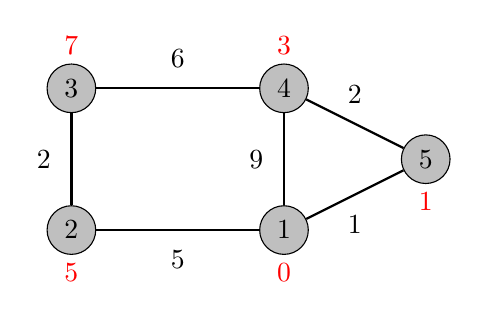
\begin{tikzpicture}[scale=0.9]
\node[draw, circle, fill=lightgray] (1) at (1,3) {3};
\node[draw, circle, fill=lightgray] (2) at (4,3) {4};
\node[draw, circle, fill=lightgray] (3) at (1,1) {2};
\node[draw, circle, fill=lightgray] (4) at (4,1) {1};
\node[draw, circle, fill=lightgray] (5) at (6,2) {5};

\node[color=red] at (1,3+0.6) {$7$};
\node[color=red] at (4,3+0.6) {$3$};
\node[color=red] at (1,1-0.6) {$5$};
\node[color=red] at (4,1-0.6) {$0$};
\node[color=red] at (6,2-0.6) {$1$};

\path[draw,thick,-] (1) -- node[font=\small,label=above:6] {} (2);
\path[draw,thick,-] (1) -- node[font=\small,label=left:2] {} (3);
\path[draw,thick,-] (3) -- node[font=\small,label=below:5] {} (4);
\path[draw,thick,-] (2) -- node[font=\small,label=left:9] {} (4);
\path[draw,thick,-] (2) -- node[font=\small,label=above:2] {} (5);
\path[draw,thick,-] (4) -- node[font=\small,label=below:1] {} (5);
\end{tikzpicture}
\end{center}


\subsubsection{Arestes negatives}

L'eficiència de l'algorisme de Dijkstra es basa en el fet que el graf
no conté arestes negatives. Si hi ha una aresta negativa l'algorisme
pot donar resultats incorrectes. Per exemple:


\begin{center}
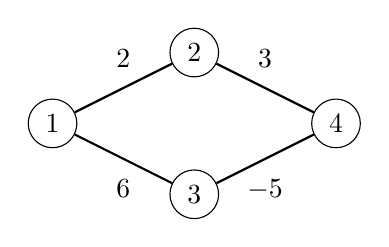
\begin{tikzpicture}[scale=0.9]
\node[draw, circle] (1) at (0,0) {$1$};
\node[draw, circle] (2) at (2,1) {$2$};
\node[draw, circle] (3) at (2,-1) {$3$};
\node[draw, circle] (4) at (4,0) {$4$};

\path[draw,thick,-] (1) -- node[font=\small,label=above:2] {} (2);
\path[draw,thick,-] (2) -- node[font=\small,label=above:3] {} (4);
\path[draw,thick,-] (1) -- node[font=\small,label=below:6] {} (3);
\path[draw,thick,-] (3) -- node[font=\small,label=below:$-5$] {} (4);
\end{tikzpicture}
\end{center}
\noindent El camí més curt des del node 1 al node 4 és $1 \rightarrow
3 \rightarrow 4$ i la seva longitud és 1. Tanmateix, l'algoritme de
Dijkstra troba el camí $1 \rightarrow 2 \rightarrow 4$ seguint les
arestes de pes mínim. L'algorisme no té en compte que en l'altre camí
el pes $-5$ serveix per compensar el pes $6$.

\subsubsection{Implementació}

La següent implementació de l'algorisme de Dijkstra calcula les
distàncies mínimes des d'un node $x$ a els altres nodes del graf. El graf
s'emmagatzema com a llistes d'adjacència de manera que
\texttt{adj[$a$]} conte un parell $(b,w)$ quan hi ha una
aresta del node $a$ fins al node $b$ amb pes $w$ .

Una implementació eficient de l'algorisme de Dijkstra requereix trobar
de manera eficient el node de distància mínima que no s'ha processat
encara. L'estructura de dades adequada és una cua de prioritats que
conté els nodes ordenats per distància. Amb una cua de prioritats
trobem el següent node a processar en temps logaritmic.

Al codi següent, la cua de prioritat \texttt{q} conté els parells de
la forma $(-d,x)$ per a indicar que la distància al node $x$ és
$d$. El vector $\texttt{distance}$ conté la distància a cada node, i
el vector $\texttt{processed}$ indica si s'ha processat un
node. Inicialment la distància és $0$ a $x$ i $\infty$ a tots els
altres nodes.


\begin{lstlisting}
for (int i = 1; i <= n; i++) distance[i] = INF;
distance[x] = 0;
q.push({0,x});
while (!q.empty()) {
    int a = q.top().second; q.pop();
    if (processed[a]) continue;
    processed[a] = true;
    for (auto u : adj[a]) {
        int b = u.first, w = u.second;
        if (distance[a]+w < distance[b]) {
            distance[b] = distance[a]+w;
            q.push({-distance[b],b});
        }
    }
}
\end{lstlisting}


Tingueu en compte que la cua de prioritat conté distàncies
\emph{negatives} als nodes. La raó d'això és que la versió
predeterminada de la cua de prioritats C++ troba els elements màxims,
mentre que volem trobar els elements mínims. Mitjançant l'ús de
distàncies negatives, podem utilitzar directament la cua de prioritat
per defecte\footnote{Per descomptat, també podríem declarar la cua de
prioritat com al capítol 4.5 i fer servir distàncies positives, però
la implementació seria una mica més llarga.}. Tingueu en compte també
que pot haver-hi diverses instàncies del mateix node a la cua de
prioritats; tanmateix, només processarem la instància amb distància
mínima.

La complexitat temporal de la implementació anterior és $O(n+m \log
m)$, perquè l'algoritme passa per tots els nodes del graf i afegeix, per
cada aresta, com a màxim una distància a la cua de prioritats.

\section{Algorisme de Floyd-Warshall}

\index{Algorisme de Floyd-Warshall}

L'algorisme de \key{Floyd–Warshall}\footnote{L'algorisme rep el nom de
R.W. Floyd i S. Warshall que el van publicar de manera independent el
1962 \cite{flo62,war62}.} proporciona una manera alternativa d'abordar
el problema de trobar els camins més curts. Aquest, a diferència dels
altres algorismes d'aquest capítol, troba tots els camins més curts
entre tots els nodes en una sola execució.

L'algorisme manté una matriu que conté les distàncies entre els
nodes. Al principi, les distàncies es calculen únicament amb arestes
directes entre els nodes, i a continuació, l'algorisme redueix les
distàncies utilitzant nodes intermedis en camins.

\subsubsection{Exemple}

Considerem com funciona l'algorisme de Floyd-Warshall al graf següent:


\begin{center}
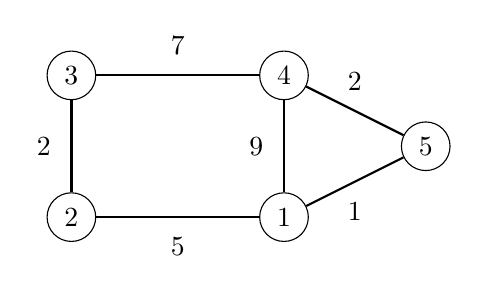
\begin{tikzpicture}[scale=0.9]
\node[draw, circle] (1) at (1,3) {$3$};
\node[draw, circle] (2) at (4,3) {$4$};
\node[draw, circle] (3) at (1,1) {$2$};
\node[draw, circle] (4) at (4,1) {$1$};
\node[draw, circle] (5) at (6,2) {$5$};

\path[draw,thick,-] (1) -- node[font=\small,label=above:7] {} (2);
\path[draw,thick,-] (1) -- node[font=\small,label=left:2] {} (3);
\path[draw,thick,-] (3) -- node[font=\small,label=below:5] {} (4);
\path[draw,thick,-] (2) -- node[font=\small,label=left:9] {} (4);
\path[draw,thick,-] (2) -- node[font=\small,label=above:2] {} (5);
\path[draw,thick,-] (4) -- node[font=\small,label=below:1] {} (5);
\end{tikzpicture}
\end{center}


Inicialment, la distància de cada node a si mateix és $0$, i la
distància entre els nodes $a$ i $b$ és $x$ si hi ha una aresta entre
els nodes $a$ i $b$ amb pes $x$. Totes les altres distàncies són
infinites.

En aquest graf, la matriu inicial és la següent:
\begin{center}
\begin{tabular}{r|rrrrr}
 & 1 & 2 & 3 & 4 & 5 \\
\hline
1 & 0 & 5 & $\infty$ & 9 & 1 \\
2 & 5 & 0 & 2 & $\infty$ & $\infty$ \\
3 & $\infty$ & 2 & 0 & 7 & $\infty$ \\
4 & 9 & $\infty$ & 7 & 0 & 2 \\
5 & 1 & $\infty$ & $\infty$ & 2 & 0 \\
\end{tabular}
\end{center}
\vspace{10pt} L'algorisme consta de rondes consecutives. A cada ronda,
l'algoritme selecciona un nou node que pot actuar com a node intermedi
en els camins a partir d'ara, i les distàncies es redueixen mitjançant
aquest node.

A la primera ronda, el node 1 és el nou node intermedi. Hi ha un nou
camí entre els nodes 2 i 4 de longitud 14, perquè el node 1 els
connecta. També hi ha un nou camí entre els nodes 2 i 5 amb longitud
6.


\begin{center}
\begin{tabular}{r|rrrrr}
 & 1 & 2 & 3 & 4 & 5 \\
\hline
1 & 0 & 5 & $\infty$ & 9 & 1 \\
2 & 5 & 0 & 2 & \textbf{14} & \textbf{6} \\
3 & $\infty$ & 2 & 0 & 7 & $\infty$ \\
4 & 9 & \textbf{14} & 7 & 0 & 2 \\
5 & 1 & \textbf{6} & $\infty$ & 2 & 0 \\
\end{tabular}
\end{center}
\vspace{10pt}

A la segona ronda, el node 2 és el nou node intermedi. Això crea nous
camins entre els nodes 1 i 3 i entre els nodes 3 i 5:


\begin{center}
\begin{tabular}{r|rrrrr}
 & 1 & 2 & 3 & 4 & 5 \\
\hline
1 & 0 & 5 & \textbf{7} & 9 & 1 \\
2 & 5 & 0 & 2 & 14 & 6 \\
3 & \textbf{7} & 2 & 0 & 7 & \textbf{8} \\
4 & 9 & 14 & 7 & 0 & 2 \\
5 & 1 & 6 & \textbf{8} & 2 & 0 \\
\end{tabular}
\end{center}
\vspace{10pt}

A la tercera ronda, el node 3 és el nou node intermedi. Hi ha un nou
camí entre els nodes 2 i 4:


\begin{center}
\begin{tabular}{r|rrrrr}
 & 1 & 2 & 3 & 4 & 5 \\
\hline
1 & 0 & 5 & 7 & 9 & 1 \\
2 & 5 & 0 & 2 & \textbf{9} & 6 \\
3 & 7 & 2 & 0 & 7 & 8 \\
4 & 9 & \textbf{9} & 7 & 0 & 2 \\
5 & 1 & 6 & 8 & 2 & 0 \\
\end{tabular}
\end{center}
\vspace{10pt}

L'algorisme continua així, fins que tots els nodes han estat designats
nodes intermedis. Un cop acabat l'algorisme, la matriu conté les
distàncies mínimes entre dos nodes qualsevol:


\begin{center}
\begin{tabular}{r|rrrrr}
 & 1 & 2 & 3 & 4 & 5 \\
\hline
1 & 0 & 5 & 7 & 3 & 1 \\
2 & 5 & 0 & 2 & 8 & 6 \\
3 & 7 & 2 & 0 & 7 & 8 \\
4 & 3 & 8 & 7 & 0 & 2 \\
5 & 1 & 6 & 8 & 2 & 0 \\
\end{tabular}
\end{center}


Per exemple, la matriu ens indica que la distància més curta entre els
nodes 2 i 4 és 8. Això correspon al camí següent:


\begin{center}
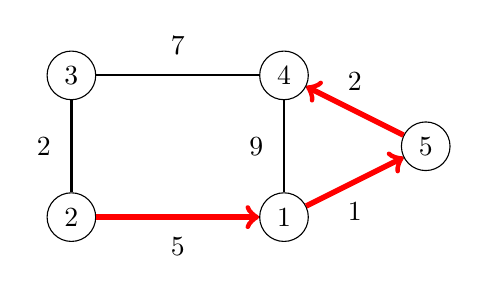
\begin{tikzpicture}[scale=0.9]
\node[draw, circle] (1) at (1,3) {$3$};
\node[draw, circle] (2) at (4,3) {$4$};
\node[draw, circle] (3) at (1,1) {$2$};
\node[draw, circle] (4) at (4,1) {$1$};
\node[draw, circle] (5) at (6,2) {$5$};

\path[draw,thick,-] (1) -- node[font=\small,label=above:7] {} (2);
\path[draw,thick,-] (1) -- node[font=\small,label=left:2] {} (3);
\path[draw,thick,-] (3) -- node[font=\small,label=below:5] {} (4);
\path[draw,thick,-] (2) -- node[font=\small,label=left:9] {} (4);
\path[draw,thick,-] (2) -- node[font=\small,label=above:2] {} (5);
\path[draw,thick,-] (4) -- node[font=\small,label=below:1] {} (5);

\path[draw=red,thick,->,line width=2pt] (3) -- (4);
\path[draw=red,thick,->,line width=2pt] (4) -- (5);
\path[draw=red,thick,->,line width=2pt] (5) -- (2);
\end{tikzpicture}
\end{center}


\subsubsection{Implementació}

L'avantatge de l'algorisme de Floyd-Warshall és que és fàcil
d'implementar. El codi següent construeix una matriu de distàncies on
$\texttt{distance}[a][b]$ és la distància més curta entre els nodes
$a$ i $b$. Primer, l'algorisme inicialitza \texttt{distance} fent
servir la matriu d'adjacència \texttt{adj} del graf:


\begin{lstlisting}
for (int i = 1; i <= n; i++) {
    for (int j = 1; j <= n; j++) {
        if (i == j) distance[i][j] = 0;
        else if (adj[i][j]) distance[i][j] = adj[i][j];
        else distance[i][j] = INF;
    }
}
\end{lstlisting}
Després d'això, les distàncies més curtes es poden trobar de la següent manera:
\begin{lstlisting}
for (int k = 1; k <= n; k++) {
    for (int i = 1; i <= n; i++) {
        for (int j = 1; j <= n; j++) {
            distance[i][j] = min(distance[i][j],
                                   distance[i][k]+distance[k][j]);
        }
    }
}
\end{lstlisting}


La complexitat temporal de l'algorisme és $O(n^3)$, perquè conté tres
bucles niats que passen per tots els nodes del graf.

Com que la implementació de l'algorisme de Floyd-Warshall és senzilla,
aquest algoritme pot ser una bona opció encara que només sigui
necessari trobar un únic camí mínim del graf. Tanmateix, l'algorisme
només pot fer-se servir quan el graf és tan petit que la complexitat
cúbica resultant és acceptable.

